%
% quadratischer_ansatz.tex
%
% (c) 2024 Flurin Brechbühler
%
\begin{figure}
    \centering
    \subfloat[Formfunktionen des quadratischen Ansatzes]{
        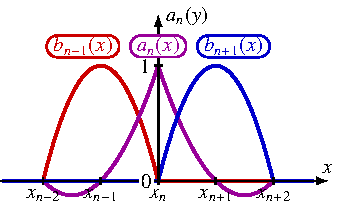
\includegraphics[scale=0.95,valign=t]{papers/fem/images/quadratisch_formfkt.pdf}
        \vphantom{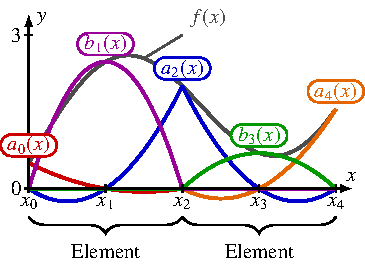
\includegraphics[width=0.45\textwidth,valign=t]{papers/fem/images/quadratisch_formfkt_skaliert.pdf}}
        \label{fem:1d:abb:quadratisch:formfkt}
    }
    \hfill
    \subfloat[Skalierte Formfunktionen mit der zu interpolierenden Funktion $f(x)$]{
        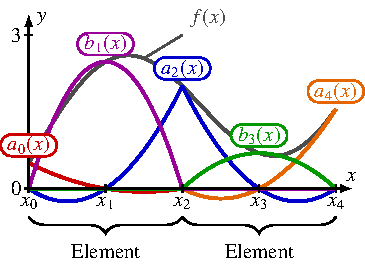
\includegraphics[scale=0.95,valign=t]{papers/fem/images/quadratisch_formfkt_skaliert.pdf}
        \vphantom{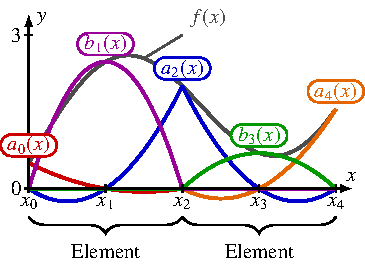
\includegraphics[width=0.45\textwidth,valign=t]{papers/fem/images/quadratisch_formfkt_skaliert.pdf}}
        \label{fem:1d:abb:quadratisch:skaliert}
    }

    \subfloat[Gegenüberstellung der interpolierten und der ursprünglichen Funktion.]{
        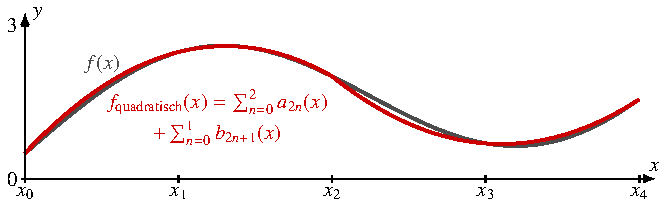
\includegraphics[scale=0.95]{papers/fem/images/quadratisch_interpoliert.pdf}
        \label{fem:1d:abb:quadratisch:vergleich}
    }
    \caption{Quadratische Interpolation des Signals $f(x)$.}
    \label{fem:1d:abb:quadratisch}
\end{figure}
    